This section elaborates on the process of radio design and steps followed to attain the results.
The focus is on determining the optimal placement of repeater stations within the network. This involves identifying strategic locations that maximise coverage while minimising the overall number of stations required.
The design approach grants the freedom to place stations at any suitable location, enabling the exploration of various configurations to achieve the desired coverage goals.
Another thing to keep in mind point-to-point microwave links operating at 28 GHz are utilised for establishing reliable connections between the repeaters.
It is important to note that the default antenna gain in \textit{Radio Mobile} is 2 dBi. However, for the purposes of this design, we must adjust the antenna gain to 0 dBi for both handheld and vehicular antennas, as per the provided instructions.

\subsection{Loading the location map}

We can load the map of the desired location in 4 different ways.
\begin{itemize}
    \item Use cursor position
    \item World Map
    \item Select a city name
    \item Enter LAT LON or QRA
\end{itemize}

\begin{wrapfigure}[9]{l}{0.45\textwidth}
\vspace{-3mm}
\centering
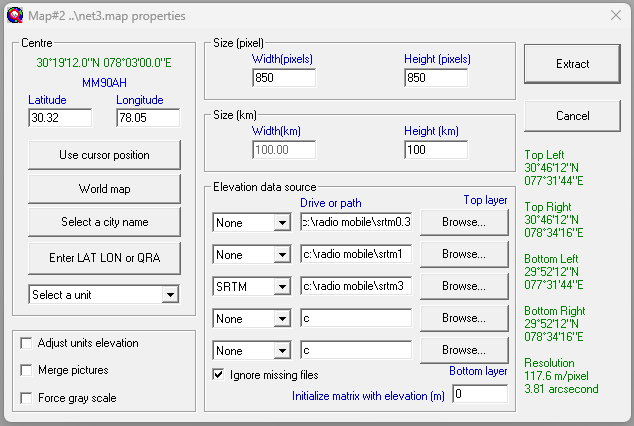
\includegraphics[width=0.35\textwidth]{Images/Map details.png}
\caption{\small Map Details}
\label{fig:MapDets}
\end{wrapfigure}

Taking advantage of the city name provided, which fortunately is included in the software's database, we can conveniently select the desired city and adjust the map scale to our preferred level of detail before loading it into the \textit{Radio Mobile} interface\cite{RadMobHndBk}.
Once the desired city is displayed on the screen, we proceed with setting up the network properties in \textit{Radio Mobile}.

\vspace{5mm}
This involves defining three distinct systems:
\begin{enumerate}
    \item \textbf{Microwave system}: Represents the point-to-point microwave links operating at 28 GHz, responsible for connecting the repeater stations.
    \item \textbf{Repeater system}: Represents the repeater stations within the network, responsible for amplifying and re-transmitting the signal.
    \item \textbf{Mobile system}: Represents the mobile users or devices within the network, receiving the signal.
\end{enumerate}
All relevant parameters for these systems is be obtained from their respective datasheets.
For all systems, omni-directional antennas are employed.
These antennas radiate signals with equal strength in all horizontal directions, making them suitable for providing coverage in all directions around the station or mobile device.

\subsection{Systems}
After defining all necessary data and parameters, the \textit{"Map Properties"} section is used to place the units within the map, ensuring optimal coverage and clearance of the first Fresnel ellipsoid.
The \textit{"Elevation"} box within \textit{Radio Mobile} provides a convenient way to determine the altitude of any selected point on the map.
For network design purposes, it's crucial to designate a specific unit as \textit{"mobile"} within the software.
This allows you to visualise and analyse the coverage area from the perspective of a mobile user.
The network structure in this case utilises a microwave point-to-point network operating at 28 GHz to connect the repeater stations.
These microwave links effectively route the signal between the repeaters.
It is important to note that stations (repeaters) can be assigned to multiple networks.
In our case, we are using four repeaters which are a part of two distinct networks, \textbf{uW\_28GHz} and \textbf{VH\_163MHz}.

\subsubsection{Microwave system}

\begin{wrapfigure}[14]{r}{0.45\textwidth}
    \vspace{-10mm}
    \centering
    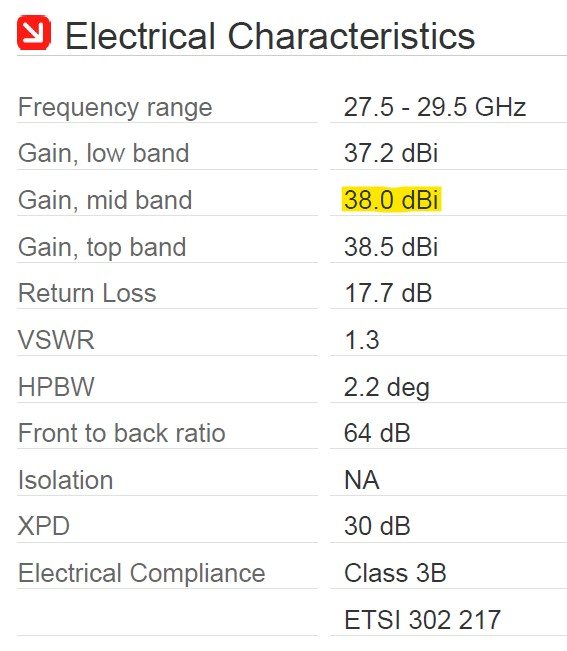
\includegraphics[width=0.35\textwidth]{Images/Antenna THP 03 275 S TX.jpg}
    \caption{\small Microwave system antenna specifications}
    \label{fig:uW_Ant}
\end{wrapfigure}

The chosen antenna for the point-to-point microwave links is the THP03275S manufactured by \textit{Faini Telecommunication Systems}\cite{THP03275S}.
This highly directional antenna boasts a significant gain of 38 dBi in the mid-band (as illustrated in figure \ref{fig:uW_Ant}), making it ideal for point-to-point communication.
Due to the narrow beamwidth, a dedicated antenna is required for each individual link.
This choice ensures uniform signal transmission in all horizontal directions, facilitating efficient communication between repeaters.
The selected microwave radio system for these systems is the PTP 820S from \textit{Cambium Networks}.

\vspace{5mm}
As per the datasheet this system operates at 28 GHz and offers a transmit power of 18 dBm and receiver sensitivity of -82.5 dBm,\cite{PTP820S} as high data rates are not a critical requirement for this application.

\begin{figure}[H]
\centering
     \begin{subfigure}[b]{0.45\textwidth}
         \centering
         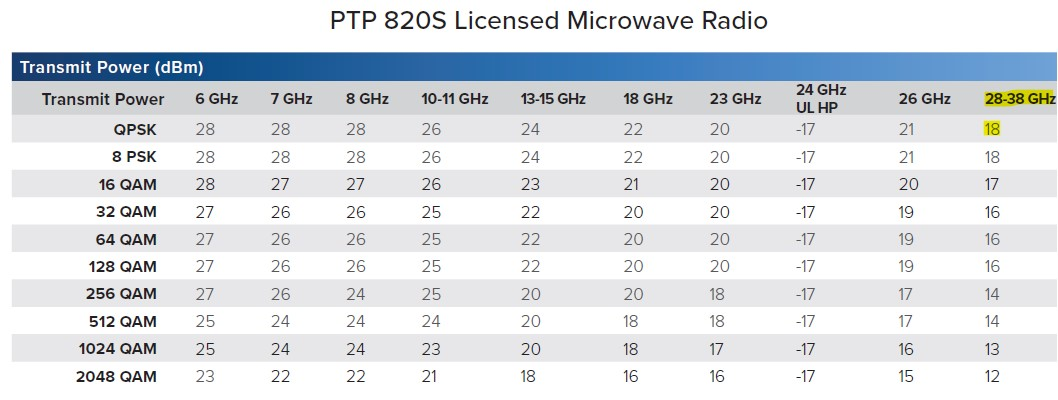
\includegraphics[width=\textwidth]{Images/PTP 820S TX.jpg}
         \caption{\small Transmitter}
         \label{fig:PTPTx}
     \end{subfigure}
     \hspace{1cm}
     \begin{subfigure}[b]{0.45\textwidth}
         \centering
         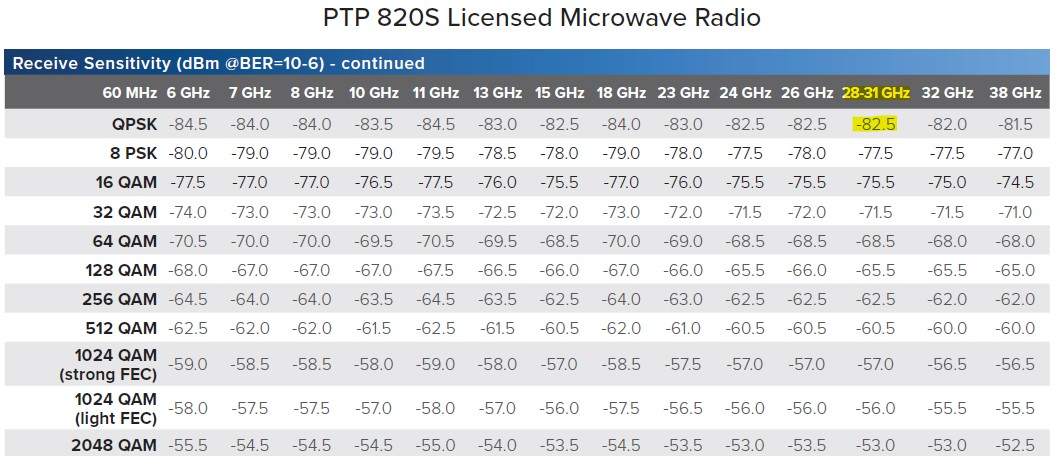
\includegraphics[width=\textwidth]{Images/PTP 820S RX.jpg}
         \caption{\small Receiver}
         \label{fig:PTPRx}
     \end{subfigure}
     \caption{Specifications of microwave system - PTP820S}
        \label{fig:PTP820S}
\end{figure}

\subsubsection{Repeater system}
The Repeater and Mobile systems both operate at 163MHz, hence it requires careful consideration of both the antenna and repeater selection.

\begin{wrapfigure}[]{l}{0.49\textwidth}
    \centering
    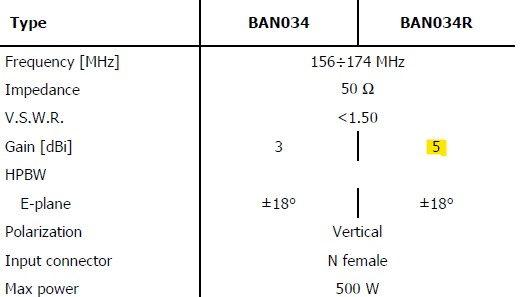
\includegraphics[width=0.49\textwidth]{Images/BAN034R - Repeater.jpg}
    \caption{\small Repeater antenna specifications}
    \label{fig:RP_Ant}
\end{wrapfigure}

Given the operating frequency, the omni-directional antenna BAN034R from \textit{BELCO Srl} was selected.
The coaxial antenna is suitable for VHF system of frequency range of 156-174MHz,as depicted in figure \ref{fig:RP_Ant} while featuring a gain of 5 dBi\cite{BAN034R}.
The chosen coaxial cable, LCF38-50J by \textit{RFS - Radio Frequency Systems}, exhibits a loss of approximately 4.89 dB/100 meter at 200MHz.
Hence, the total line loss is around 0.5 dB for an antenna 10 meters from the repeater.

\begin{figure}[H]
\centering
     \begin{subfigure}[b]{0.45\textwidth}
         \centering
         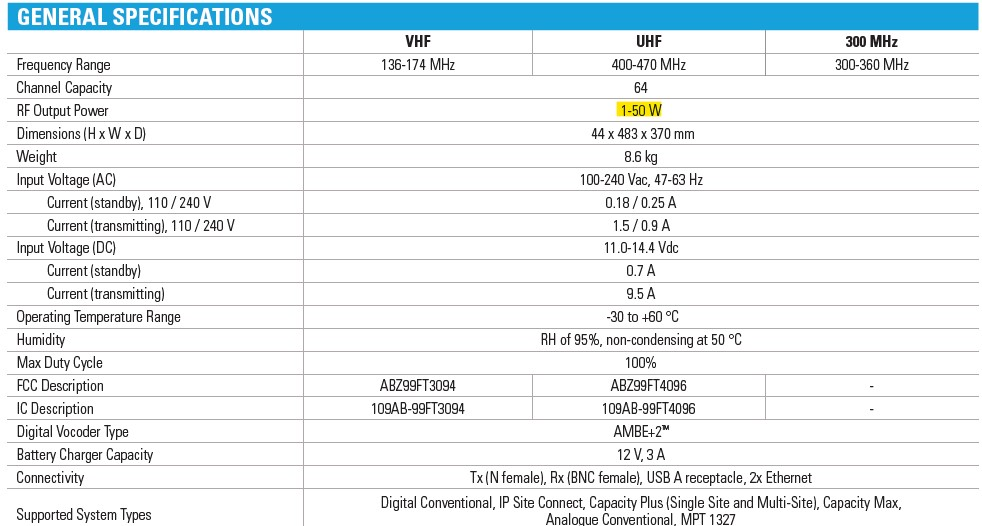
\includegraphics[width=\textwidth]{Images/SLR5500 TX.jpg}
         \caption{\small Transmitter}
         \label{fig:SLRTx}
     \end{subfigure}
     \hspace{1cm}
     \begin{subfigure}[b]{0.45\textwidth}
         \centering
         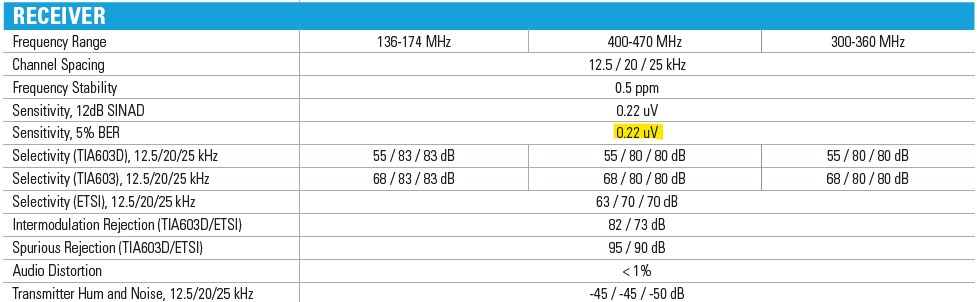
\includegraphics[width=\textwidth]{Images/SLR5500 RX.jpg}
         \caption{\small Receiver}
         \label{fig:SLRRx}
     \end{subfigure}
     \caption{Specifications of repeater system - SLR5500}
        \label{fig:SLR5500}
\end{figure}

For the repeater module, we were instructed (as per the problem statement) to use Motorola SLR 5500 by \textit{Motorola Solutions}.
It boasts an RF output power ranging from 1 to 50W, although for this specific system, we chose to go with an average value of 25W.
Additionally, as seen in the figure \ref{fig:SLRRx}, it possesses a receive sensitivity of 0.16µV.

\subsubsection{Mobile System}
The mobile unit within the \textit{VHF\_163MHz} network, is using the DM4000E by \textit{Motorola Solutions}, which is is configured with a transmit power of 25 W and receiver sensitivity is set to 0.18 $\mu$V.
Following the problem statement, the mobile device is assumed to have an antenna with a gain of 0 dB and a low antenna height of approximately 2 metres.

\begin{figure}[H]
\centering
     \begin{subfigure}[b]{0.45\textwidth}
         \centering
         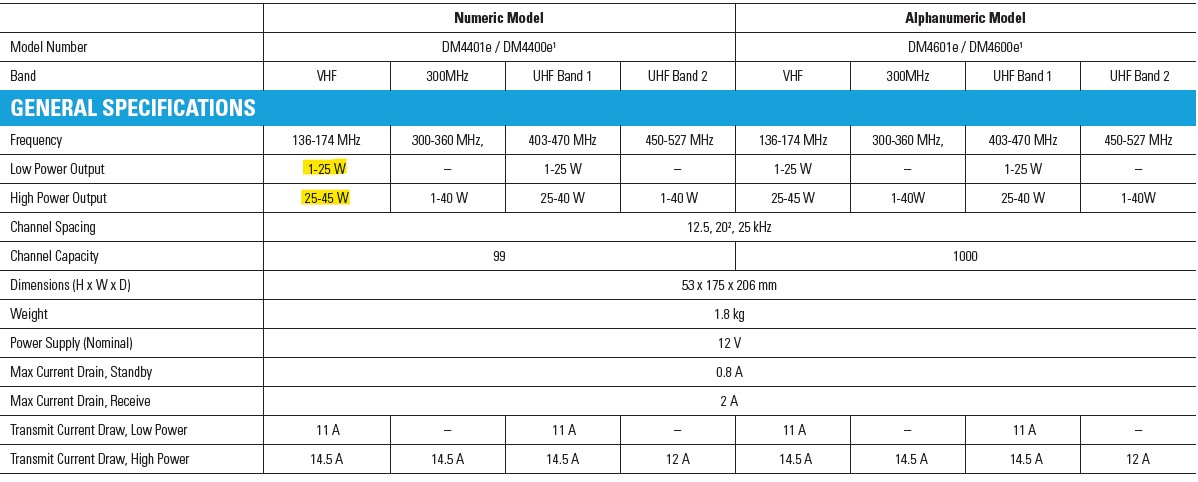
\includegraphics[width=\textwidth]{Images/DM4000E TX.jpg}
         \caption{\small Transmitter}
         \label{fig:DM4KETx}
     \end{subfigure}
     \hspace{1cm}
     \begin{subfigure}[b]{0.45\textwidth}
         \centering
         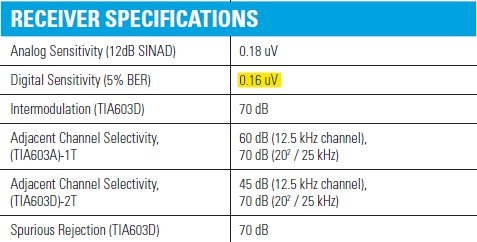
\includegraphics[width=\textwidth]{Images/DM4000E RX.jpg}
         \caption{\small Receiver}
         \label{fig:DM4KERx}
     \end{subfigure}
     \caption{Specifications of mobile system - DM4000E}
        \label{fig:DM4000E}
\end{figure}